% !TeX spellcheck = en_US
% !TeX encoding = UTF-8 

\documentclass[12pt,a4paper]{article}

% document language, encoding and geometry
\usepackage[english]{babel}
\usepackage[utf8x]{inputenc}
\usepackage[a4paper,
			margin=0.85in]{geometry}
\usepackage{setspace}

% styling file
\usepackage{kprjHSE} 

% packages for math environments and graphics
\usepackage{amsmath}
\usepackage{amssymb}
\usepackage{amsthm}
\usepackage{graphicx} 

% table package, allows for various table shapes and cell colors
\usepackage{xcolor}
\usepackage{tabularray}

% packages for code listing
\usepackage{listings}
\usepackage{courier}
\lstset{
	showstringspaces=false,
	inputencoding=utf8x, 
	extendedchars=\true,
	language=python,
	frame=single,
	basicstyle=\ttfamily,
	breaklines=true,
	tabsize=4
}

% misc. packages
\usepackage{cite}
\usepackage{subfigure}

\homeworkHSE

\FirstAuthor{M.~Kirdin}
\SecondAuthor{V.~Kropotin}
\ThirdAuthor{V.~Pendishchuk}
\discipline{Basic Methods of Data Analysis}
\faculty{Faculty of Computer Science}
\chair{School of Data Analysis and Artificial Intelligence}
\chief{B.~Mirkin}
\workyear{2024}

\onehalfspacing

\begin{document}
	
	\maketitle
	
	\tableofcontents
	
	\section{Data}
	
	\subsection{Description}
	
	We chose the Diamonds Price Dataset since it has a variety of easily interpretable features (see \figref{fig:sample}) as well as an abundance of data. It has 50,000 entities and 10 features, which are:
	\begin{itemize}
		\itemsep 0pt
		\item \textbf{Carat.} Weight of a diamond, carats (quantitative).
		\item \textbf{Cut.}	Cutting quality (categorical).
		\item \textbf{Color.} Color from J (worst) to D (best) (categorical).
		\item \textbf{Clarity.} Clarity from left to right is worst to best: I1, SI2, SI1, VS2, VS1, VVS2, VVS1, IF (categorical).
		\item \textbf{x.} Length, mm (quantitative).
		\item \textbf{y.} Width, mm (quantitative).
		\item \textbf{z.} Depth, mm (quantitative).
		\item \textbf{depth.} Percentage depth z/(mean(x,y)), \% (quantitative).
		\item \textbf{table.} Width of the widest point at the top of the diamond, mm (quantitative).
		\item \textbf{price.} Diamond's price (quantitative).
	\end{itemize}
	
	\begin{figure}[hbtp]
		\centering
		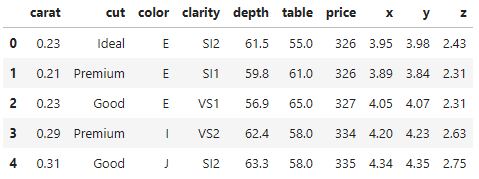
\includegraphics[width=.75\textwidth]{media/sample.png}
		\caption{Sample data from the Diamonds Price Dataset}
		\label{fig:sample}
	\end{figure}
	
	\subsection{Preprocessing}
	
	In this work we considered a sample of 2,000 entities from  this dataset, since it contains enough data to derive nontrivial relations in data while not being demanding in terms of computational power. Since all categorical features imply some sort of order in their values, it was decided to use ordinal encoding by assigning different integer values to different classes in ascending order from worst to best. Furthermore, in most calculations standard scaling was used to center and normalize the data.
	
	\section{Correlation coefficient}
	
	\subsection{Pairwise distributions}
	
	To understand which pair of features is the best for constructing a linear regression on, we have to take into account their distributions. As shown on \figref{fig:pairplot}, there are several features of interest: "x", "y", "z", "carat" and "price". Features "x", "y" and "z", with the exception of some outliers, are distributed in a linear pattern and their distributions wrt "carat" look like polynomial functions. This is an expected behavior, since "carat" is roughly the product of "x", "y", "z", which are linearly distributed with each other, and diamond density. 
	
	\begin{figure}[hbtp]
		\centering
		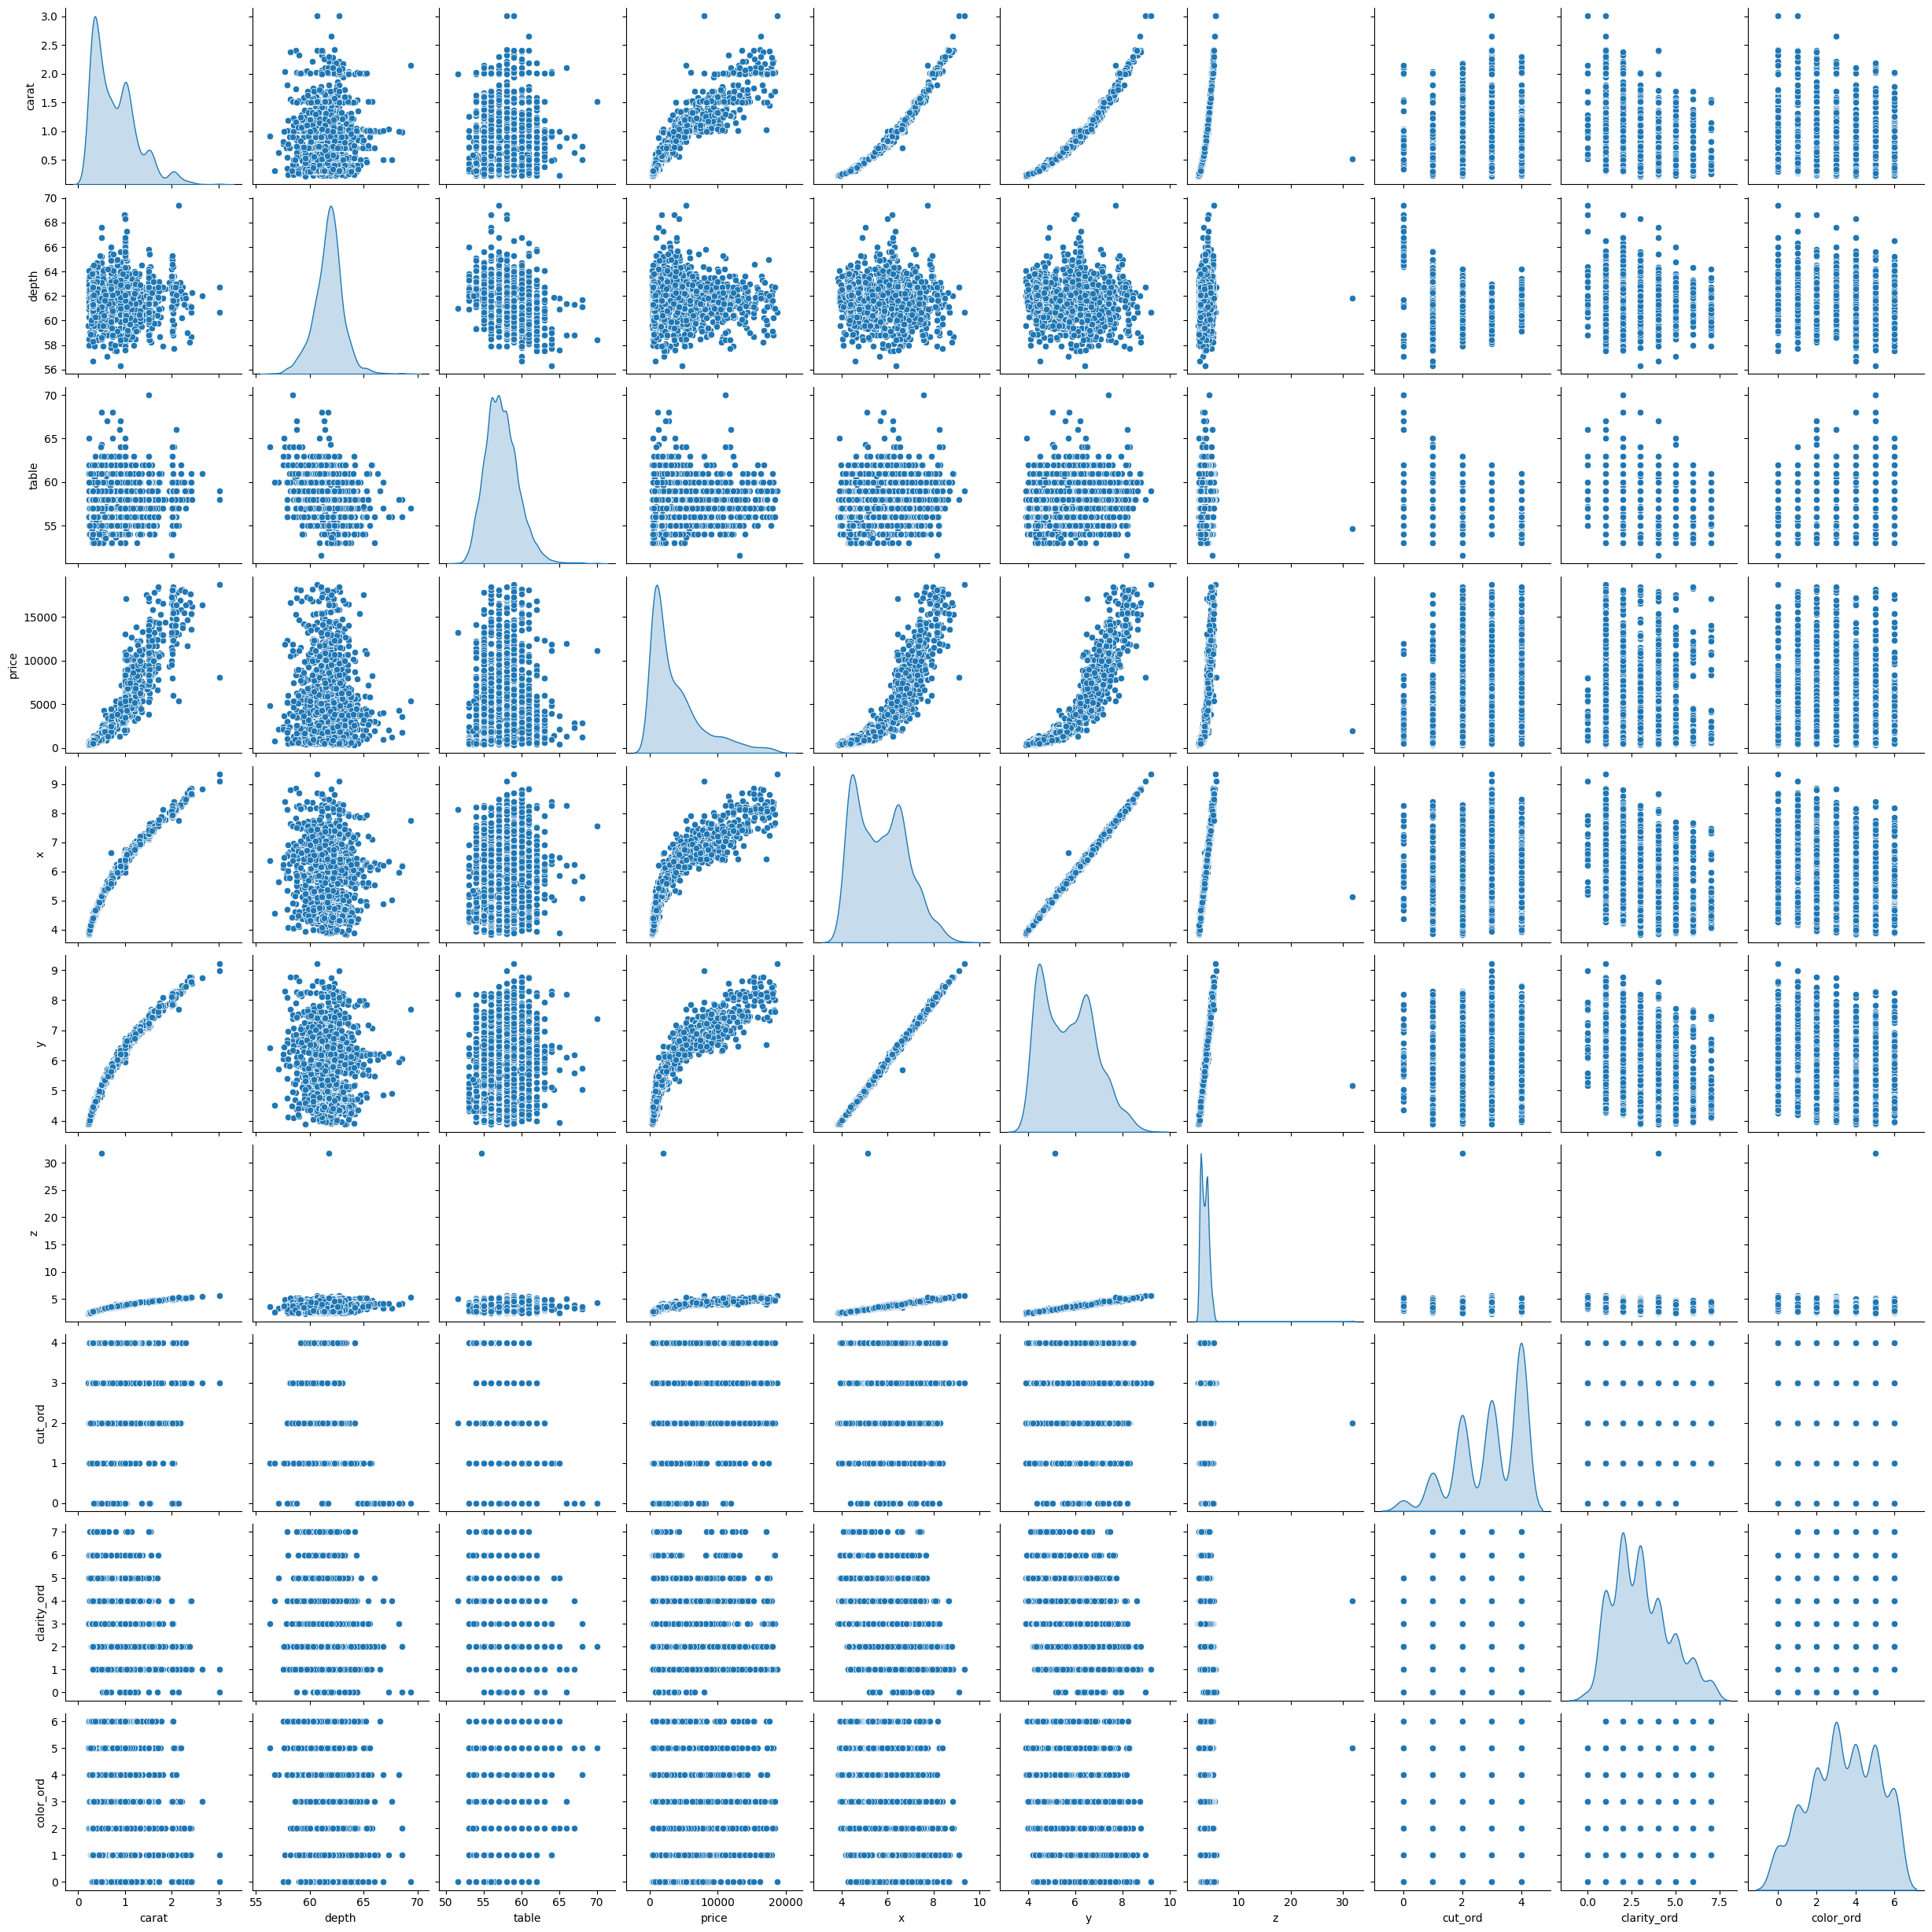
\includegraphics[width=.95\textwidth]{media/pairplot.png}
		\caption{Pairwise scatter plots of all the features in data}
		\label{fig:pairplot}
	\end{figure}
	
	\newpage
	
	\subsection{Linear regression}
	
	In this task we will consider the pair "carat" and "price", because their distribution is not as trivial as those of diamonds' physical dimensions wrt each other or their mass (\figref{fig:caratVprice}).
	
	\begin{figure}[h]
		\centering
		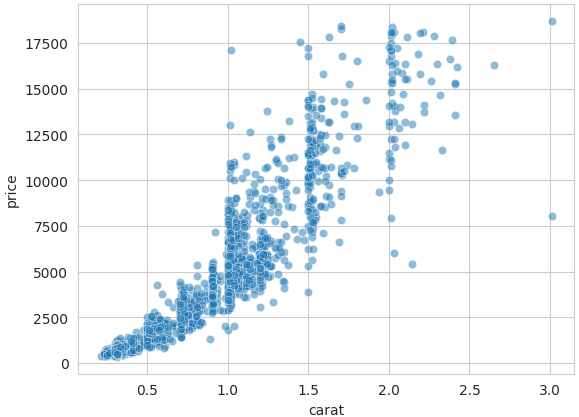
\includegraphics[width=.6\textwidth]{media/caratVprice.png}
		\caption{Distribution "carat" and "price" wrt each other}
		\label{fig:caratVprice}
	\end{figure}
	
	First, a regular linear regression of "price" over "carat" was constructed. As shown on \figref{fig:caratVpriceReg}, this line has a positive slope, hence the diamond's price tends to positively correlate with its mass, which is to be expected. Next, the correlation and $R^2$ coefficient, also known as \textit{the coefficient of determination}, were computed:
	\[\rho = 0.9240,\, R^2 = 0.8537.\]
	
	\begin{figure}[h]
		\centering
		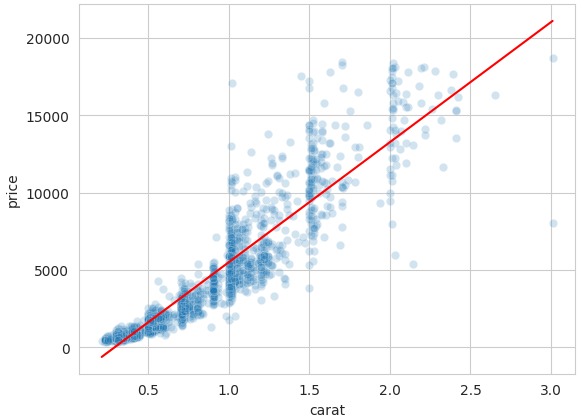
\includegraphics[width=.6\textwidth]{media/caratVpriceReg.png}
		\caption{Linear regression of "price" over "carat"}
		\label{fig:caratVpriceReg}
	\end{figure}
	
	\newpage
	
	Since $R^2$ coefficient is the proportion of variance of the target feature taken into account by linear regression, in our case  $85.37\%$ of "price" variance is taken into account.
	
	After that, a set 
	\[x=\begin{pmatrix}
			0.3000 & 863\\
			0.3100 & 788\\
			0.4000 & 662\\ 
			2.0100 & 17078
		\end{pmatrix}\]
	of four random pairs of "carat" and "price" values was chosen to compare the predicted and true "price" values. To do this, the percentile deviations were found:
	\begin{multline*}
	\Delta{}y_{\text{true}} = \left(89.9245\%,\, 79.1276\%,\, -30.2385\%,\, 21.8683\%\right)^T,\\ \Delta{}y_{\text{pred}}=\left(892.5046\%,\, 379.1018\%,\, -23.2178\%,\, 27.9890\%\right)^T,
	\end{multline*}
	where $\Delta{}y_{\text{true}}$ is relative deviation of predicted from true values and $\Delta{}y_{\text{pred}}$ is the other way round. From this we can conclude that the regression line tends to underestimate the price of diamonds with lower mass.
	
	Finally, mean absolute percentile error(MAPE) relative to both true and predicted over the whole data was considered in order to measure the mean deviation of the data from the predictor line and vice versa:
	\[\text{MAPE}_{\text{true}}= 39.2063\%,\, \text{MAPE}_{\text{pred}}=121.4897\%.\]
	These values indicate that, similarly to the previous case, regression on this pair features tends to underestimate the "price" feature. There is also another interpretation: $\text{MAPE}_{\text{true}}$ is data analysis(DA) view on MAPE, while $\text{MAPE}_{\text{pred}}$ is machine learning(ML) view on MAPE; hence, while in terms of DA the line we constructed is good, while the opposite is true in terms of ML.
	
	\begin{figure}[h]
		\centering
		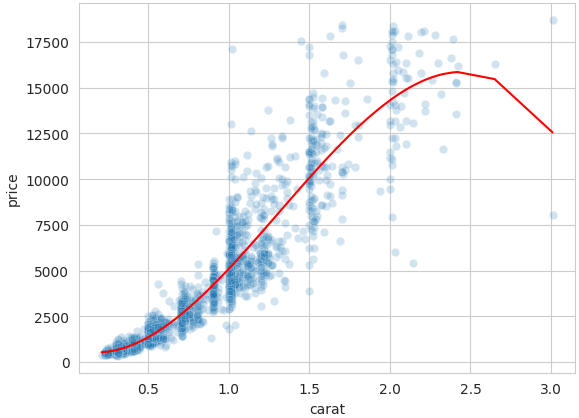
\includegraphics[width=.56\textwidth]{media/caratVpriceRegAlt.png}
		\caption{Polynomial regression of "price" over "carat"}
		\label{fig:caratVpriceRegAlt}
	\end{figure}
	
	\newpage
	We also tried polynomial regression with a third degree polynomial, as seen on \figref{fig:caratVpriceRegAlt}. This resulting in following MAPE values:
	\[\text{MAPE}_{\text{true}}= 39.2063\%,\, \text{MAPE}_{\text{pred}}=37.0984\%.\]
	This indicates that the polynomial curve uses more data and does not underestimate the price.
	
	\section{PCA/SVD}
	
	For principal component analysis (PCA), the following subset of features was considered: x, y, z, depth, table, carat. These features were chosen for the following reasons:
	\begin{itemize}
		\itemsep 0pt
		\item These features are all continuous, and that makes them easier to interpret as coordinates in a linear space, as opposed to categorical features.
		\item These features all relate to the same aspect - the size of a diamond: x, y, z and table describe the dimensions of a diamond, depth is a ratio calculated from the main dimensions, and carat is a diamond's weight.
		\item All features, except depth, correlate to some extent with each other (\figref{fig:pcaCorr}).
	\end{itemize}
	
	\begin{figure}[hbtp]
		\centering
		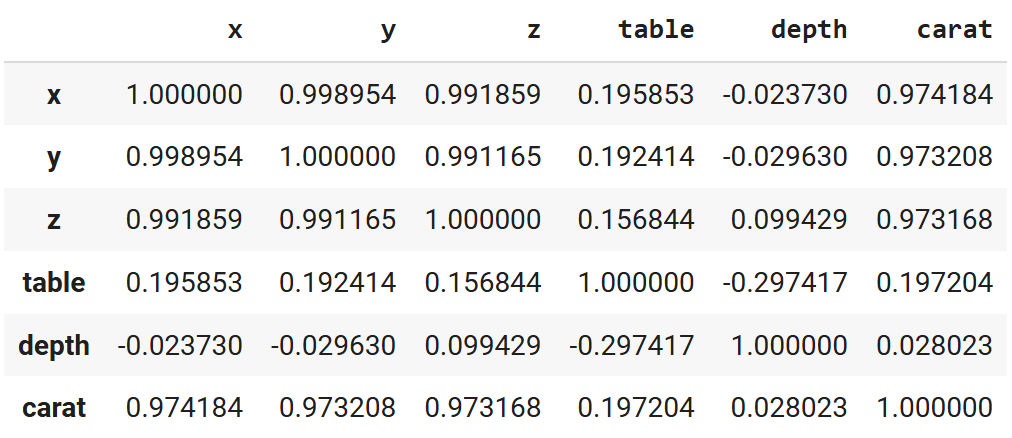
\includegraphics[width=.7\textwidth]{media/pcaCorr.png}
		\caption{Correlation matrix for the features chosen for PCA}
		\label{fig:pcaCorr}
	\end{figure}
	
	\newpage
	
	The data was standardized using three different techniques covered in class, resulting in three different datasets:
	\begin{itemize}
		\itemsep 0pt
		\item z-scoring:
		\[y_{iv} = \frac{x_{iv} - mean_v}{std_v} \]
		\item range normalization:
		\[y_{iv} = \frac{x_{iv} - mean_v}{max_v - min_v}\]
		\item ranking normalization:
		\[y_{iv} = \frac{x_{iv} - min_v}{max_v - min_v}\]
	\end{itemize}
	
	After standardization, singular value decomposition (SVD) was computed for the three standardized datasets and the original subset of the dataset, with the latter added for the sake of comparison. From the obtained decomposition results, data scatter and principal component contributions were computed.
	
	\begin{center}
		\noindent \textbf{Table 1.} SVD results for the non-standardized data
		\vspace{1em}
		
		\begin{tblr}{width=\linewidth,
				vline{0,1-10}={1-19}{0.5pt},
				hline{0,1-19}={1-10}{0.5pt}}
			\SetCell[r=1, c=9]{c}{Data scatter: 2875588.8702}\\
			
			\SetCell[r=2, c=1]{c}{Singular\\value $\sigma_v$} & \SetCell[r=2, c=1]{c}{Natural\\contribution} & \SetCell[r=2, c=1]{c}{Contribution\\\%} & \SetCell[r=1, c=6]{c}{Singular vector\\components (loadings)} \\
			& & & x & y & z & table & depth & carat\\
			1694.9 & 2872698.57 & 100. & -0.067 & -0.067 & -0.041 & -0.679 & -0.727 & -0.009\\
			41.3 & 1706.5 & 0. & 0.213 & 0.212 & 0.103 & 0.667 & -0.669 & 0.087\\
			34.3 & 1177.21 & 0. & 0.588 & 0.583 & 0.372 & -0.307 & 0.155 & 0.242\\
			2.2 & 4.99 & 0. & -0.203 & -0.273 & 0.153 & 0.016 & 0.009 & 0.928\\
			1. & 1.09 & 0. & -0.119 & -0.326 & 0.898 & 0.017 & -0.022 & -0.270\\
			0.7 & 0.5 & 0. & -0.741 & 0.656 & 0.142 & 0.003 & -0.003 & 0.008
		\end{tblr}
	\end{center}
	
	\bigskip
	
	\begin{center}
		\noindent \textbf{Table 2.} SVD results for the z-scoring standardized data
		\vspace{1em}
		
		\begin{tblr}{width=\linewidth,
				vline{0,1-10}={1-19}{0.5pt},
				hline{0,1-19}={1-10}{0.5pt}}
			\SetCell[r=1, c=9]{c}{Data scatter: 2394.}\\
			
			\SetCell[r=2, c=1]{c}{Singular\\value $\sigma_v$} & \SetCell[r=2, c=1]{c}{Natural\\contribution} & \SetCell[r=2, c=1]{c}{Contribution\\\%} & \SetCell[r=1, c=6]{c}{Singular vector\\components (loadings)} \\
			& & & x & y & z & table & depth & carat\\
			39.9 & 1594.93 & 66.62 & 0.498 & 0.498 & 0.496 & 0.123 & -0.000 & 0.493\\
			22.6 & 512.65 & 21.41 & 0.012 & 0.010 & 0.103 & -0.668 & 0.736 & 0.040\\
			16.5 & 271.48 & 11.34 & 0.078 & 0.087 & -0.003 & -0.733 & -0.669 & 0.020\\
		\end{tblr}
	\end{center}
	
	\newpage
	
	\begin{center}
		\noindent \textbf{Table 2.} (continued)
		\vspace{1em}
		
		\begin{tblr}{width=\linewidth,
				vline{0,1-10}={1-19}{0.5pt},
				hline{0,1-19}={1-10}{0.5pt}}
			\SetCell[r=2, c=1]{c}{Singular\\value $\sigma_v$} & \SetCell[r=2, c=1]{c}{Natural\\contribution} & \SetCell[r=2, c=1]{c}{Contribution\\\%} & \SetCell[r=1, c=6]{c}{Singular vector\\components (loadings)} \\
			& & & x & y & z & table & depth & carat\\
			3.8 & 14.4 & 0.6 & 0.280 & 0.293 & 0.282 & 0.022 & 0.019 & -0.869\\
			0.6 & 0.4 & 0.02 & 0.730 & -0.683 & -0.039 & -0.004 & 0.000 & -0.008\\
			0.4 & 0.14 & 0.01 & -0.367 & -0.439 & 0.814 & -0.001 & -0.103 & -0.004\\
		\end{tblr}
	\end{center}
	
	\bigskip
	
	\begin{center}
		\noindent \textbf{Table 3.} SVD results for the range standardized data
		\vspace{1em}
		
		\begin{tblr}{width=\linewidth,
				vline{0,1-10}={1-19}{0.5pt},
				hline{0,1-19}={1-10}{0.5pt}}
			\SetCell[r=1, c=9]{c}{Data scatter: 84.7789}\\
			
			\SetCell[r=2, c=1]{c}{Singular\\value $\sigma_v$} & \SetCell[r=2, c=1]{c}{Natural\\contribution} & \SetCell[r=2, c=1]{c}{Contribution\\\%} & \SetCell[r=1, c=6]{c}{Singular vector\\components (loadings)} \\
			& & & x & y & z & table & depth & carat\\
			8.2 & 66.5 & 78.43 & 0.524 & 0.537 & 0.513 & 0.093 & 0.001 & 0.407\\
			3.5 & 12.38 & 14.6 & 0.018 & 0.020 & 0.103 & -0.906 & 0.410 & 0.025\\
			2.3 & 5.43 & 6.4 & 0.084 & 0.101 & -0.100 & -0.413 & -0.896 & -0.017\\
			0.7 & 0.45 & 0.53 & 0.226 & 0.248 & 0.229 & 0.024 & 0.030 & -0.913\\
			0.1 & 0.02 & 0.02 & 0.730 & -0.683 & -0.020 & -0.005 & -0.004 & -0.011\\
			0.1 & 0.01 & 0.01 & -0.367 & -0.415 & 0.815 & -0.001 & -0.171 & -0.005
		\end{tblr}
	\end{center}
	
	\bigskip
	
	\begin{center}
		\noindent \textbf{Table 4.} SVD results for the ranking standardized data
		\vspace{1em}
		
		\begin{tblr}{width=\linewidth,
				vline{0,1-10}={1-19}{0.5pt},
				hline{0,1-19}={1-10}{0.5pt}}
			\SetCell[r=1, c=9]{c}{Data scatter: 3600976.1901}\\
			
			\SetCell[r=2, c=1]{c}{Singular\\value $\sigma_v$} & \SetCell[r=2, c=1]{c}{Natural\\contribution} & \SetCell[r=2, c=1]{c}{Contribution\\\%} & \SetCell[r=1, c=6]{c}{Singular vector\\components (loadings)} \\
			& & & x & y & z & table & depth & carat\\
			1794.6 & 3220431.16 & 89.43 & -0.446 & -0.452 & -0.436 & -0.409 & -0.408 & -0.270\\
			505.8 & 255844.96 & 7.1 & -0.288 & -0.306 & -0.268 & 0.558 & 0.586 & -0.310\\
			343.3 & 117845.97 & 3.27 & -0.021 & -0.025 & 0.091 & -0.718 & 0.689 & -0.023\\
			77.4 & 5992.18 & 0.17 & 0.296 & 0.322 & 0.048 & -0.061 & -0.079 & -0.893\\
			25.9 & 672.25 & 0.02 & 0.342 & 0.335 & -0.853 & -0.046 & 0.093 & 0.183\\
			13.8 & 189.67 & 0.01 & 0.716 & -0.697 & 0.010 & -0.005 & -0.010 & -0.012
		\end{tblr}
	\end{center}
	
	\newpage
	
	From the table 1 one can see the enormous scatter of non-standardized data. This is likely due to the different features scales (\figref{fig:pcaDesc}) - while the diamond size dimensions x, y, z and the weight in carats are in single digits, table and depth have average values of 57.5 and 61.6 respectively. When squared, table and depth contribute greatly to the data scatter, exceeding the contributions of other features many times over. This affects the results of PCA, as can be seen from the 100\% contribution of the first principal component in Table 1. Therefore, the use of standardization is essential in order to properly apply PCA to the given data.
	
	\begin{figure}[hbtp]
		\centering
		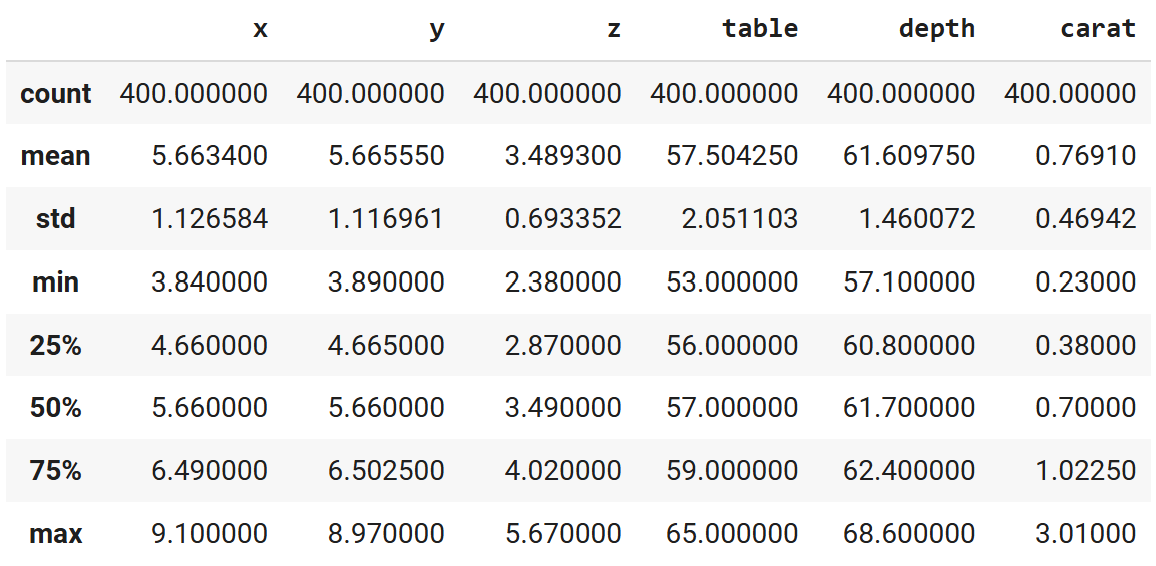
\includegraphics[width=.7\textwidth]{media/pcaDesc.png}
		\caption{Descriptive statistics for the features chosen for PCA}
		\label{fig:pcaDesc}
	\end{figure}
	
	The data scatter for ranking standardized data is also worth mentioning, as it is even greater than that of non-standardized data. This may be explained by the fact that most of the features chosen for PCA follow normal distribution, and thus, when ranking normalization is applied, most of the values in the dataset become large values close to 50. In general, SVD for ranking normalization has shown to produce results similar to those for non-standardized data, which suggests a high degree of information loss due to how features are distributed.
	
	As an example, let us describe the results in the table 2. Here one can see that the summary contribution of the first two principal components to the data scatter equals $66.62 + 21.41 = 88.03\%$, with the first principal component contributing the most. From the loading components it can be seen the first principal component is positively correlated with x, y, z, table and carat and negatively correlated with depth. While the first component's correlations with table and depth is positive and negative respectively, the second component's correlations with the same features is inverted. From singular vector values, the first component is generally greater when diamond's dimensions and weight are higher. Thus, intuitively, the first component corresponds to how "large" a diamond is.
	
	After data preprocessing, the first two principal components obtained via SVD were visualized for two normalization methods - z-scoring and range normalization (\figref{fig:pcaComp}). Additionally, two groups of diamonds were considered to help facilitate the understanding of\newline
	\newpage
	\noindent  these visualizations. These groups are:
	
	\begin{enumerate}
		\itemsep 0pt
		\item Diamonds with large weight in carats (carat $>$ 2.1).
		\item Diamonds with low depth ratios (depth $<$ 58.5).
	\end{enumerate}
	
	
	The thresholds that define the groups were determined from the distribution graphs of corresponding features (\figref{fig:depthDist}, \oldref{fig:caratDist}).
	
	\begin{figure}[hbtp]
		\centering
		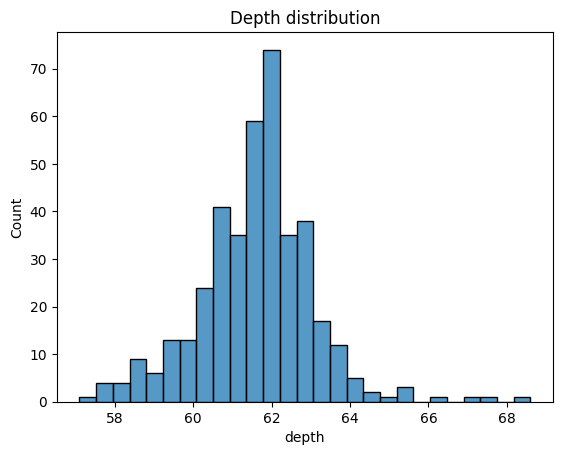
\includegraphics[width=.5\textwidth]{media/depthDist.png}
		\caption{Depth feature distribution}
		\label{fig:depthDist}
	\end{figure}
	
	\begin{figure}[hbtp]
		\centering
		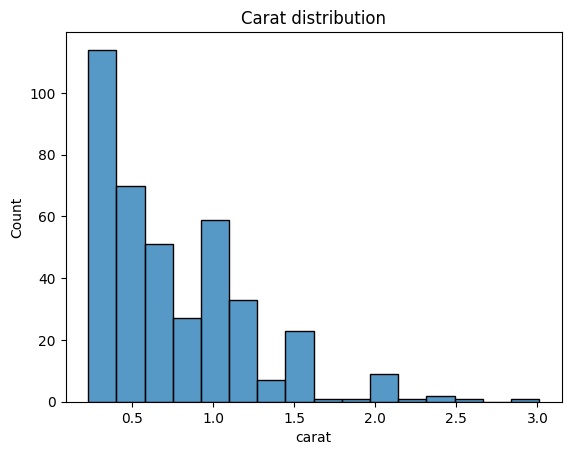
\includegraphics[width=.5\textwidth]{media/caratDist.png}
		\caption{Carat feature distribution}
		\label{fig:caratDist}
	\end{figure}
	
	Overall, the visualizations for both normalization techniques share many similarities in the overall distribution of instances. The most noticeable difference is that the visualizations are flipped vertically - the signs of the second principal component coordinates on these two visualizations are opposites. This is merely the result of us flipping the signs in accordance to the largest loading values to make the visualizations prettier. Another notable difference is that instances on the left are a bit more scattered along the second principal component axis. This can be attributed to greater data scatter contribution of the second principal component for z-standardized data (21.41\% vs. 14.6\% for z-scoring and range normalization respectively).
	
	Due to the fact that most features (x, y, z, depth, table) follow normal distribution, and carat seems to follow the Pareto distribution (the Matthew principle), z-scoring seems to be more suitable for the given data.
	
	As for the groups, it seems that larger weight in carat coincides with larger values of the first principal component, while smaller depth ratios coincide with lesser second principal component values. This follows from the observation that both groups seem to denote the outliers in the respective axes.
	
	\begin{figure}[hbtp]
		\centering
		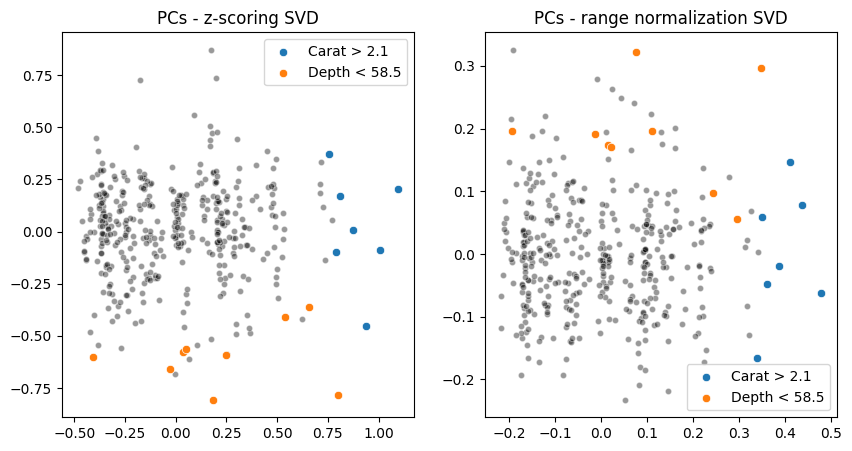
\includegraphics[width=.7\textwidth]{media/pcaComp.png}
		\caption{Visualizations of the first two principal components for z-scoring and range normalization}
		\label{fig:pcaComp}
	\end{figure}
	
	\begin{figure}[hbtp]
		\centering
		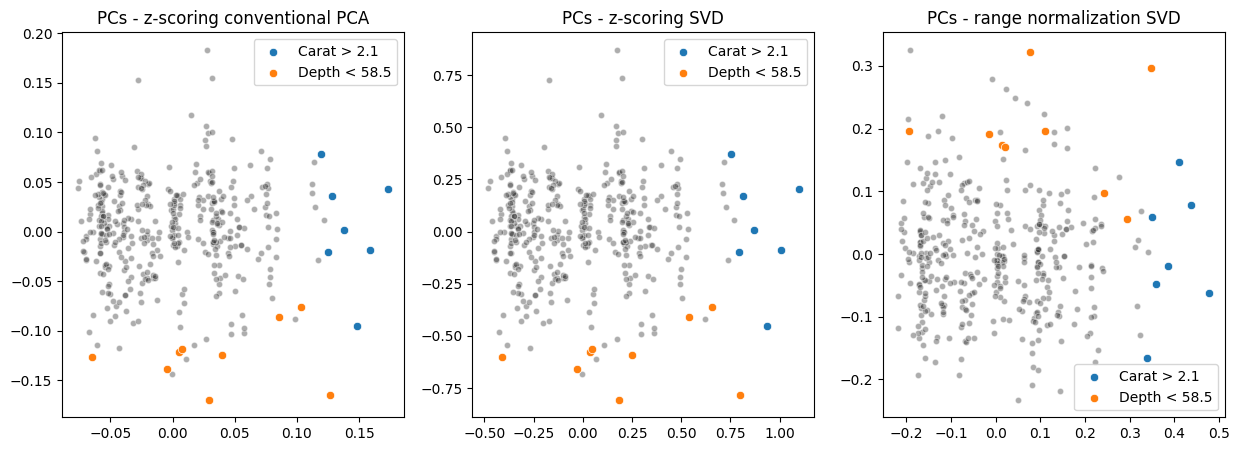
\includegraphics[width=.9\textwidth]{media/pcaConvComp.png}
		\caption{Visualizations of the first two principal components computed with SVD and conventional PCA}
		\label{fig:pcaConvComp}
	\end{figure}
	
	Comparing the visualizations obtained for the SVD-based PCA approach with the visualization obtained for the conventional PCA approach on z-standardized data on \figref{fig:pcaConvComp}, one can see that the visualizations corresponding to z-standardized data are virtually the same, with the only difference being different scales. Thereafter, the visualizations of the two groups are also in the same positions.
	
	Looking at the hidden factor ranking in table 5, it is easy to see that the score is naturally correlated with diamond's dimensions and weight. Intuitively it follows that the hidden factor describes how large a diamond is.
	
	\begin{center}
		\noindent \textbf{Table 5.} Top 10 instances by their hidden score
		\vspace{1em}
		
		\begin{tblr}{
				cells = {c},
				hlines,
				vlines,
			}
			\textbf{x} & \textbf{y} & \textbf{z} & \textbf{carat} & \textbf{table} & \textbf{depth} & \textbf{score} \\
			9.10       & 8.97       & 5.67       & 3.01           & 58.0           & 62.7           & 100.000000     \\
			8.82       & 8.75       & 5.45       & 2.65           & 61.0           & 62.0           & 98.484294      \\
			8.85       & 8.76       & 5.17       & 2.41           & 61.0           & 58.7           & 89.666102      \\
			8.60       & 8.56       & 5.24       & 2.33           & 58.0           & 61.1           & 86.891979      \\
			8.33       & 8.28       & 5.21       & 2.22           & 58.0           & 62.7           & 86.601659      \\
			7.89       & 7.81       & 5.04       & 2.00           & 60.0           & 64.2           & 86.520889      \\
			7.97       & 7.86       & 5.03       & 2.04           & 60.0           & 63.6           & 86.141693      \\
			8.22       & 8.30       & 5.08       & 2.11           & 60.0           & 61.5           & 86.105723      \\
			8.22       & 8.16       & 5.10       & 2.08           & 59.0           & 62.3           & 85.170271      \\
			8.39       & 8.31       & 4.82       & 2.04           & 64.0           & 57.7           & 84.878480      
		\end{tblr}
	\end{center}
	
	\section{Cluster analysis and cluster interpretation}
	
	To understand the general pricing patterns a following subset of features was explored via K-Means algorithm:
	\begin{itemize}
		\itemsep 0pt
		\item "depth";
		\item "table";
		\item "carat";
		\item "price".
	\end{itemize}
	These features denote the physical parameters of a diamond and were scaled to have normal distribution before the clustering algorithm was applied to them. 
	
	Then, using the build-in K-Means algorithm with 4 and 7 clusters were applied to the data. It was initialized to start with twelve sets of random centers for each number of clusters used. Algorithm's performance was measured with inertia metric:
	\[L = \sum\limits_{k=1}^{K}\sum\limits_{i\in S_{k}}\sum\limits_{v\in V} \left(y_{iv} - c_{kv}\right)^2,\]
	where $K$ is the number of clusters;
	
	$S_k$ is the number of objects in $k$-th cluster;
	
	$V$ is the set of features;
	
	$y_{iv}$ is value of feature $v$ of the $i$-th object from cluster $k$;
	
	$c_{kv}$ is value of feature $v$ of the center of cluster $k$.
	
	After the evaluation, for each number of clusters the best-performing cluster set was chosen for further analysis. On those the absolute and relative deviations from grand mean for each feature were calculated: 
	\[d_{abs}=(c_{kv}-c_{v}),\, d_{rel}=\dfrac{c_{kv}-c_{v}}{c_v}\cdot100\%.\]
	For each cluster in each table deviations in a feature of more than 30\% were marked with green(positive deviations) and red(negative deviation) backgrounds. 
	
	\begin{center}
		\noindent \textbf{Table 6.} Best set for K-Means with 4 clusters\\
		\begin{tblr}{width=\linewidth,
			vline{0,1-6}={1-19}{0.5pt},
			hline{0,1-19}={1-6}{0.5pt}}
			 & \textbf{depth} & \textbf{table} & \textbf{carat} & \textbf{price}\\
			 
			grand mean & 61.7409 & 57.3868 & 0.7865 & 3858.1980\\
			 
			\SetCell[r=1, c=5]{c}{\textbf{cluster 1 (234 instances)}}\\
			center & 61.4547 & 58.0838 & \SetCell{green8}1.6865 & \SetCell{green8}12463.5812\\
			grand mean devation & -0.2861 & 0.6970 & \SetCell{green8}0.9000 & \SetCell{green8}8605.3832\\
			rel. grand mean deviation & -0.46\% & 1.21\% & \SetCell{green8}114.44\% & \SetCell{green8}223.04\%\\
		\end{tblr}
	\end{center}
	
	\begin{center}
		\noindent \textbf{Table 6.} (continued)\\
		\begin{tblr}{width=\linewidth,
				vline{0,1-6}={1-19}{0.5pt},
				hline{0,1-19}={1-6}{0.5pt}}
			& \textbf{depth} & \textbf{table} & \textbf{carat} & \textbf{price}\\
			
			grand mean & 61.7409 & 57.3868 & 0.7865 & 3858.1980\\
			
			\SetCell[r=1, c=5]{c}{\textbf{cluster 2 (854 instances)}}\\
			center & 62.0034 & 56.1681 & \SetCell{red9}0.4438 & \SetCell{red8}1276.4660\\
			grand mean devation & 0.2625 & -1.2187 & \SetCell{red9}-0.3427 & \SetCell{red8}-2581.7320\\
			rel. grand mean deviation & 0.43\% & -2.12\% & \SetCell{red9}-43.57\% & \SetCell{red8}-66.92\%\\
			
			\SetCell[r=1, c=5]{c}{\textbf{cluster 3 (512 instances)}}\\
			center & 62.5969 & 57.3387 & \SetCell{green9}1.0456 & \SetCell{green9}5258.8340\\
			grand mean devation & 0.8560 & -0.0481 & \SetCell{green9}0.2592 & \SetCell{green9}1400.6360\\
			rel. grand mean deviation & 1.39\% & -0.08\% & \SetCell{green9}32.95\% & \SetCell{green9}36.30\%\\
			
			\SetCell[r=1, c=5]{c}{\textbf{cluster 4 (400 instances)}}\\
			center & 60.2520 & 59.6425 & 0.6599 & \SetCell{red9}2543.2325\\
			grand mean devation & -1.4889 & 2.2557 & -0.1266 & \SetCell{red9}-1314.9655\\
			rel. grand mean deviation & -2.41\% & 3.93\% & -16.10\% & \SetCell{red9}-34.08\%
		\end{tblr}
	\end{center}
			
	According to the table 6, those four clusters correspond to extremely valuable, extremely cheap, moderately valuable and moderately cheap diamonds respectively. Interestingly, "depth" and "table" do not deviate that much from their respective grand means and do not correlate with neither "price" nor "carat".
	
	Similar conclusion can be made for the case with 7 clusters. As shown on the table 7, they correspond to various "price" and "mass" ranges with clusters in similar range being divided based on their "depth" and "table" deviations.
	
	\begin{center}
		\noindent \textbf{Table 7.} Best set for K-Means with 7 clusters\\
		\begin{tblr}{width=\linewidth,
				vline{0,1-6}={1-27}{0.5pt},
				hline{0,1-27}={1-6}{0.5pt}}
			& \textbf{depth} & \textbf{table} & \textbf{carat} & \textbf{price}\\
			
			grand mean & 61.7409 & 57.3868 & 0.7865 & 3858.1980\\
			
			\SetCell[r=1, c=5]{c}{\textbf{cluster 1 (193 instances)}}\\
			center & 61.5523 & 58.2466 & \SetCell{green8}1.7496 & \SetCell{green8}13071.0829\\
			grand mean devation & -0.1885 & 0.8598 & \SetCell{green8}0.9631 & \SetCell{green8}9212.8849\\
			rel. grand mean deviation & -0.31\% & 1.50\% & \SetCell{green8}122.46\% & \SetCell{green8}238.79\%\\
			
			\SetCell[r=1, c=5]{c}{\textbf{cluster 2 (290 instances)}}\\
			center & 60.5655 & 57.3117 & \SetCell{red9}0.4779 & \SetCell{red8}1450.8103\\
			grand mean devation & -1.1753 & -0.0751 & \SetCell{red9}-0.3085 & \SetCell{red8}-2407.3877\\
			rel. grand mean deviation & -1.90\% & -0.13\% & \SetCell{red9}-39.23\% & \SetCell{red8}-62.40\%\\
		\end{tblr}
	\end{center}
	\newpage
	\begin{center}
		\noindent \textbf{Table 7.} (continued)\\
		\begin{tblr}{width=\linewidth,
				vline{0,1-6}={1-27}{0.5pt},
				hline{0,1-27}={1-6}{0.5pt}}
			& \textbf{depth} & \textbf{table} & \textbf{carat} & \textbf{price}\\
			
			grand mean & 61.7409 & 57.3868 & 0.7865 & 3858.1980\\
			
			\SetCell[r=1, c=5]{c}{\textbf{cluster 3 (350 instances)}}\\
			center & 62.3123 & 58.0829 & \SetCell{red8}0.4388 & \SetCell{red8}1231.0829\\
			grand mean devation & 0.5714 & 0.6961 & \SetCell{red8}-0.3476 & \SetCell{red8}-2627.1151\\
			rel. grand mean deviation & 0.93\% & 1.21\% & \SetCell{red8}-44.20\% & \SetCell{red8}-68.09\%\\
			
			\SetCell[r=1, c=5]{c}{\textbf{cluster 4 (192 instances)}}\\
			center & 59.7719 & 60.8776 & 0.8353 & 3704.7188\\
			grand mean devation & -1.9690 & 3.4908 & 0.0488 & -153.4792\\
			rel. grand mean deviation & -3.19\% & 6.08\% & 6.21\% & -3.98\%\\
			
			\SetCell[r=1, c=5]{c}{\textbf{cluster 5 (184 instances)}}\\
			center & 63.7891 & 58.3761 & 1.0024 & 4422.3478\\
			grand mean devation & 2.0483 & 0.9893 & 0.2159 & 564.1498\\
			rel. grand mean deviation & 3.32\% & 1.72\% & 27.45\% & 14.62\%\\
			
			\SetCell[r=1, c=5]{c}{\textbf{cluster 6 (431 instances)}}\\
			center & 62.1624 & 55.0935 & \SetCell{red8}0.4575 & \SetCell{red8}1338.5963\\
			grand mean devation & 0.4216 & -2.2933 & \SetCell{red8}-0.3290 & \SetCell{red8}-2519.6017\\
			rel. grand mean deviation & 0.68\% & -4.00\% & \SetCell{red8}-41.83\% & \SetCell{red8}-65.31\%\\
			
			\SetCell[r=1, c=5]{c}{\textbf{cluster 7 (360 instances)}}\\
			center & 61.7317 & 56.6878 & \SetCell{green8}1.1141 & \SetCell{green8}6222.5278\\
			grand mean devation & -0.0092 & -0.6990 & \SetCell{green8}0.3277 & \SetCell{green8}2364.3298\\
			rel. grand mean deviation & -0.01\% & -1.22\% & \SetCell{green8}41.66\% & \SetCell{green8}61.28\%\\
		\end{tblr}
	\end{center}
	
	Overall, "depth" and "table" seem to have no correlation to both the diamond's price and its mass. Increasing the number of classes seems to subdivide the price ranges into smaller pieces determined by their "table" and "depth".
	
	\section{Contingency Table}
	
	\subsection{Feature selection}
	
	Let's select the price feature and make it binarized according to the following criteria: $0-1000$, $1000-2500$, $2500-5000$, $5000-10000$, $10000+$. For the second feature, we will choose the clustering into 4 classes obtained in the previous paragraph, and we will work with these two categorical features.
	
	\subsection{Contingency table}
		
	To calculate the Contingency table, let's calculate how many elements fell into each pair from the Cartesian product of the binarized cluster price (the results are presented in Table 8).
	
	\begin{center}
		\noindent \textbf{Table 8.} Contingency table
		\begin{tblr}{width=\linewidth,
				vline{0,1-6}={1-19}{0.5pt},
				hline{0,1-19}={1-6}{0.5pt}}
			bin-price/cluster & \textbf{cluster 1} & \textbf{cluster 2} & \textbf{cluster 3}& \textbf{cluster 4}\\
			
			$0-1000$ & 465 & 119 & 1 & 0 \\
			$1000-2500$ & 302 & 131 & 25 & 0 \\
			$2500-5000$ & 79 & 98 & 233 & 0 \\
			$5000-10000$ & 2 & 58 & 247 & 45 \\
			$10000+$ & 0 & 1 & 7 & 187 \\
			
		\end{tblr}
	\end{center}
	
	Now let's calculate the conditional probabilities, to do this, calculate the sum of the matrix from Table 8 by columns and rows, respectively, and divide the matrices into the calculated total statistics, taking into account the dimensions. The results are presented in Tables 9 and 10, respectively.
	
	Values where the probability is greater than $70\%$ are marked in green, and probabilities greater than $50\%$ but less than $70\%$ are blue. In Table 9, the probability of $80.6\%$ (marked in green) shows that belonging to cluster 4 entails the probability of $80.6\%$ that the price is more than 10,000. It also follows from belonging to cluster 1 that the price will be in the range from 0 to 1000 with a probability of $54.83\%$ (marked in blue). In Table 10, belonging to the price categories of $0-1000$ and $1000-2500$ entails a high probability of belonging to 1 cluster ($79.49\%$ and $65.94\%$), for average prices ($2500-5000$ and $5000-10000$) there is a high probability of 3 clusters of $56.83\%$ and $70.17\%$ respectively. And with almost a single probability ($95.9\%$), if an element has a price of more than 10,000, then it belongs to the 4th cluster.
	
	Thus, we can conclude that clusters are very strongly related to the price, and the higher the cluster number, the higher the prices and vice versa.
	
	Next, we calculate the Quetelet indices, the results are presented in Table 11 (colors indicate statistically significant results, green is greater than 0.3, red is less than -0.3). It can be concluded that low price values are associated with cluster 1 (as we noted above), and negatively affect clusters 3,4. And medium and high prices give a positive boost to clusters 3 and 4, respectively.
	
	\subsection{Average Quetelet index and Pearson’s chi-squared}
	
	We calculate $Q$ and $\varphi$ using formulas, the implementation of which can be found in the Appendix A,
	$Q=sum(sum(pq)) = 1.3181$, $\varphi = sum(sum([(pab-pi).*(pab-pi)]./pi)) = 1.3181$. We get that phi-squared value is equal to the average Quetelet index.
	
	\subsection{Confidence level}
	
	$\chi^2 = 2000\cdot1.3181 = 2636.2685$. This is a high value which provides for rejection of the hypothesis of independence at both $95\%$ and $99\%$ confidence levels. Since we have 5 and 4 unique values for the features, we get $(5-1)(4-1)=12$ degrees of freedom, and the critical chi squared values for $95\%$ and $99\%$ are $21.0$ and $26.2$, respectively. To reject the independence hypothesis in either case, one needs the number of objects greater than $\dfrac{21.0}{\varphi}=15.93$ and greater than $\dfrac{26.2}{\varphi}=19.87$, that are 16 and 20, respectively.
	
	
	\begin{center}
		\noindent \textbf{Table 9.} column-conditional probabilities
		\begin{tblr}{width=\linewidth,
				vline{0,1-6}={1-19}{0.5pt},
				hline{0,1-19}={1-6}{0.5pt}}
			bin-price/cluster & \textbf{cluster 1} & \textbf{cluster 2} & \textbf{cluster 3}& \textbf{cluster 4}\\
			
			$0-1000$ & \SetCell{blue8}0.5483 & 0.2924 & 0.0019& 0. \\
			$1000-2500$ & 0.3561 & 0.3219 & 0.0487 & 0. \\
			$2500-5000$ & 0.0932 & 0.2408 & 0.4542 & 0. \\
			$5000-10000$ & 0.0024 & 0.1425 & 0.4815 & 0.194 \\
			$10000+$ & 0.    & 0.0025& 0.0136& \SetCell{green8}0.806 \\
			
		\end{tblr}
	\end{center}
	
	\bigskip
	
	\begin{center}
		\noindent \textbf{Table 10.} row-conditional probabilities
		\begin{tblr}{width=\linewidth,
				vline{0,1-6}={1-19}{0.5pt},
				hline{0,1-19}={1-6}{0.5pt}}
			bin-price/cluster & \textbf{cluster 1} & \textbf{cluster 2} & \textbf{cluster 3}& \textbf{cluster 4}\\
			
			$0-1000$ & \SetCell{green8}0.7949 & 0.2034 & 0.0017 & 0. \\
			$1000-2500$ & \SetCell{blue8}0.6594 & 0.286 & 0.0546 & 0. \\
			$2500-5000$ & 0.1927 & 0.239 & \SetCell{blue8}0.5683& 0. \\
			$5000-10000$ & 0.0057& 0.1648& \SetCell{green8}0.7017& 0.1278 \\
			$10000+$ & 0.    & 0.0051 & 0.0359& \SetCell{green8}0.959 \\
			
		\end{tblr}
	\end{center}
	
	\bigskip
	
	\begin{center}
		\noindent \textbf{Table 11.} Quetelet indices
		\begin{tblr}{width=\linewidth,
				vline{0,1-6}={1-19}{0.5pt},
				hline{0,1-19}={1-6}{0.5pt}}
			bin-price/cluster & \textbf{cluster 1} & \textbf{cluster 2} & \textbf{cluster 3}& \textbf{cluster 4}\\
			
			$0-1000$ & \SetCell{green8}0.8747 & -0.0004 & \SetCell{red8}-0.9933 & \SetCell{red8}-1. \\
			$1000-2500$ & \SetCell{green8}0.5552 &  \SetCell{green8}0.4055 & \SetCell{red8}-0.7872& \SetCell{red8}-1. \\
			$2500-5000$ & \SetCell{red8}-0.5456 &  0.1746 &  \SetCell{green8}1.2156 & \SetCell{red8}-1. \\
			$5000-10000$ & \SetCell{red8}-0.9866 & -0.1903 &  \SetCell{green8}1.7357 &  0.1021 \\
			$10000+$ & \SetCell{red8}-1.    & \SetCell{red8}-0.9748& \SetCell{red8}-0.86  &  \SetCell{green8}7.267 \\
			
		\end{tblr}
	\end{center}
	
	
	\section{Bootstrapping}
	
	\begin{center}
		\noindent \textbf{Table 12.} Characteristics of clusters 3 and 4, grand mean
		\begin{tblr}{width=\linewidth,
				vline{0,1-6}={1-19}{0.5pt},
				hline{0,1-19}={1-6}{0.5pt}}
			& \textbf{Mean} & \textbf{Standard deviation}\\
			
			grand mean & 57.3868 & 2.1540 \\
			cluste 3 & 57.3263 & 1.7518 \\
			cluste 4 & 58.1060 & 2.0878 \\
			
		\end{tblr}
	\end{center}
	
	\begin{center}
		\noindent \textbf{Table 13.} Bootstrapping results for table, $95\%$ confidence intervals
		\begin{tblr}{width=\linewidth,
				vline{0,1-6}={1-19}{0.5pt},
				hline{0,1-19}={1-6}{0.5pt}}
			& \textbf{left bound} & \textbf{right bound}\\
			
			grand mean (pivotal)& 57.2925 & 57.4814 \\
			grand mean (non-pivotal)& 57.2997 & 57.4843 \\
			grand mean - mean in cluster 3 (pivotal)& -0.117 & 0.237 \\
			grand mean - mean in cluster 3 (non-pivotal)& -0.114 & 0.236 \\
			mean in cluster 3 - mean in cluster 4 (pivotal)& -1.089 & -0.471 \\
			mean in cluster 3 - mean in cluster 4 (non-pivotal)& -1.095 & -0.458 \\
			
		\end{tblr}
	\end{center}
	
	\begin{figure}[hbtp]
		\centering
		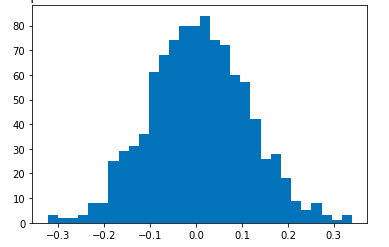
\includegraphics[width=.8\textwidth]{media/grand_mean_bootstrup.png}
		\caption{Bootstrap of ground mean of "table"}
		\label{fig:grand_mean_bootstrup}
	\end{figure}
	
	\subsection{Confidence interval for grand mean of table}
	
	We chose the "table" feature and clusters 3 and 4, because for this feature, the average in the two selected clusters is very close to the overall average for the entire dataset. In Table 13, the first two lines show the results of calculating the $95\%$ confidence interval for the "table" feature across the entire sample (the whole sample distribution presented in \figref{fig:grand_mean_bootstrup} with 4000 iterations in bootstrap). As you can see, since the number of observations in the sample is large (2000), the results of pivotal and non-pivotal methods give very close estimates on the boundaries of the confidence interval.
	
	\begin{figure}[h]
		\centering
		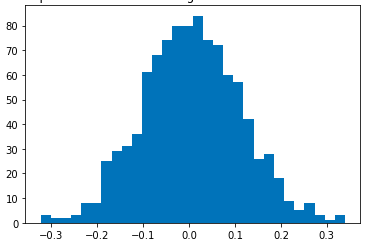
\includegraphics[width=.8\textwidth]{media/grand_mean_cluster_3.png}
		\caption{Bootstrap of difference between grand mean and mean in cluster 3 of "table" feature}
		\label{fig:grand_mean_cluster3_bootstrup}
	\end{figure}
	
	\subsection{Comparison of means in two selected clusters}
	
	As you can see from Table 12, the average in cluster 3 is slightly less than the average in cluster 4, as well as the standard deviation. From the last two rows of Table 13, we can conclude that the average in cluster 3 is statistically significantly less than the average in cluster 4 for the significance level of $5\%$, since the $95\%$ confidence interval does not include $0$ (this is done for both pivotal and non-pivotal approaches). A bootstrapped sample for the difference in averages between cluster 3 and cluster 4 is presented in \figref{fig:grand_mean_cluster3_bootstrup} with 4000 iterations in bootstrap). The distribution is quite symmetrical, but the part of the distribution near the value of $-0.1$ has a density higher than the symmetrical part near to $0.1$, which creates a slight bias on average in the negative direction (the average in cluster 3 is less than the average in cluster 4).
	
	\subsection{Testing hypothesis that mean in cluster 3 coincide with grand mean}
	
	Let's choose cluster 3, since the average value of the "table" feature within this cluster is closest to the average of the entire sample. To test the hypothesis of the equality of the two averages using bootstrap at the $5\%$ significance level, we need to look at the confidence interval for the difference built using bootstrap. As can be seen from Table 13 (lines 3 and 4), for both approaches, pivotal and non-pivotal, the confidence interval contains $0$, which means that the null hypothesis of equality of averages does not deviate at the $5\%$ significance level. In \figref{fig:cluster3_cluster4_bootstrup} you can see the distribution of bootstrap difference between mean in cluster 3 and mean in cluster 4.
	
	\begin{figure}[hbtp]
		\centering
		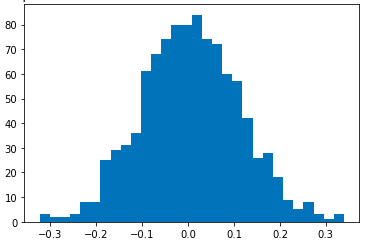
\includegraphics[width=.8\textwidth]{media/cluster_3_cluster_4.png}
		\caption{Bootstrap of difference between mean in cluster 3 and mean in cluster 4}
		\label{fig:cluster3_cluster4_bootstrup}
	\end{figure}
	
	\section*{Appendix A}
	\addcontentsline{toc}{section}{\MakeUppercase{Appendix A}}
	\begin{center}
		\noindent\textbf{Listing A.1} Data preprocessing, correlation matrix, K-Means.
	\end{center}
	\lstinputlisting[language=Python, showstringspaces=false]{listings/corr_kmeans.py}
	\newpage
	\begin{center}
		\noindent\textbf{Listing A.2} PCA/SVD.
	\end{center}
	\begin{lstlisting}
	import numpy as np
	import pandas as pd
	import seaborn as sns
	import matplotlib.pyplot as plt
	
	SEED = 42
	np.random.seed(SEED)
	
	np.set_printoptions(suppress=True)
	
	# !curl -L -o diamonds-price-dataset.zip https://www.kaggle.com/api/v1/datasets/download/amirhosseinmirzaie/diamonds-price-dataset
	# !unzip diamonds-price-dataset.zip
	
	"""# Dataset & feature selection"""
	
	N = 400
	df = pd.read_csv('diamonds.csv').sample(n=N, random_state=SEED)
	
	print("Shape:", df.shape)
	df.head()
	
	"""Features chosen: `x`, `y`, `z`, `table`, `depth` and `carat`. All of these features describe the size of a diamond."""
	
	data = df[['x', 'y', 'z', 'table', 'depth', 'carat']]
	
	data.head()
	
	data.describe()
	
	data.corr()
	
	"""# Data standardization"""
	
	means = data.mean(axis=0)
	means
	
	stds = data.std(axis=0)
	stds
	
	ranges = data.max(axis=0) - data.min(axis=0)
	ranges
	
	# Z-score normalization
	data_zs = (data - means) / stds
	
	# Range normalization
	data_rd = (data - means) / ranges
	
	# Ranking normalization
	data_rn = 100.0 * (data - data.min(axis=0)) / ranges
	
	# Performing singular value decomposition
	uzs, szs, vzs = np.linalg.svd(data_zs)
	urd, srd, vrd = np.linalg.svd(data_rd)
	urn, srn, vrn = np.linalg.svd(data_rn)
	uns, snss, vns = np.linalg.svd(data)
	
	print("Singular values for z-score normalization:", szs.round(1))
	print("Singular values for range normalization:", srd.round(1))
	print("Singular values for ranking normalization:", srn.round(1))
	print("Singular values for no standardization:", snss.round(1))
	
	contrib_zs = np.square(szs)
	contrib_rd = np.square(srd)
	contrib_rn = np.square(srn)
	contrib_ns = np.square(snss)
	
	print("PC natural contributions (z-score normalization):", contrib_zs.round(2))
	print("PC natural contributions (range normalization):", contrib_rd.round(2))
	print("PC natural contributions (ranking normalization):", contrib_rn.round(2))
	print("PC natural contributions (no standardization):", contrib_ns.round(2))
	
	ds_zs = np.square(data_zs).to_numpy().sum()
	ds_rd = np.square(data_rd).to_numpy().sum()
	ds_rn = np.square(data_rn).to_numpy().sum()
	ds_ns = np.square(data).to_numpy().sum()
	
	print("Data scatter by definition (z-score normalization): %.4f" % ds_zs)
	print("Data scatter by definition (range normalization): %.4f" % ds_rd)
	print("Data scatter by definition (ranking normalization): %.4f" % ds_rn)
	print("Data scatter by definition (no standardization): %.4f" % ds_ns)
	
	ds_contib_zs = contrib_zs.sum()
	ds_contib_rd = contrib_rd.sum()
	ds_contib_rn = contrib_rn.sum()
	ds_contib_ns = contrib_ns.sum()
	
	print("Data scatter from contributions (z-score normalization): %.4f" % ds_contib_zs)
	print("Data scatter from contributions (range normalization): %.4f" % ds_contib_rd)
	print("Data scatter from contributions (ranking normalization): %.4f" % ds_contib_rn)
	print("Data scatter from contributions (no standardization): %.4f" % ds_contib_ns)
	
	"""From the results one can see that the calculated data scatter is the same for all versions of standardization, which is consistent with the theory."""
	
	contrib_zs_percent = 100.0 * contrib_zs / ds_zs
	contrib_rd_percent = 100.0 * contrib_rd / ds_rd
	contrib_rn_percent = 100.0 * contrib_rn / ds_rn
	contrib_ns_percent = 100.0 * contrib_ns / ds_ns
	
	print("PC percentage contributions (z-score normalization):", contrib_zs_percent.round(2))
	print("PC percentage contributions (range normalization):", contrib_rd_percent.round(2))
	print("PC percentage contributions (ranking normalization):", contrib_rn_percent.round(2))
	print("PC percentage contributions (no standardization):", contrib_ns_percent.round(2))
	
	for i in range(6):
	x_arrstr = np.char.mod('%.3f', vrn[i].round(3))
	#combine to a string
	print(" & ".join(x_arrstr))
	
	vzs
	
	"""Here we see that the contrast between principle component contributions is  starker for range normalization - 78% PC1 contribution for r-standardization vs. 67% PC1 contribution for z-standardization.
	
	Ranking normalization brings PC1 contribution even further up to 89%, closer to the non-standardizaed contribution distribution.
	
	# Principal components visualization
	
	For the purpose of visualizing two first principal components and the differences between them, let us use two features to define two separate groups of dataset instances: `depth` and `carat`.
	
	The first group are diamonds with small depth ratios (< 58.5, as shown below). The second group are diamonds of large weight (> 2.1 carats, as shown below).
	
	## Defining instance groups
	"""
	
	sns.histplot(data['depth']).set_title('Depth distribution')
	
	# Diamonds with small depth ratios
	depth_group = df[df['depth'] < 58.5]
	depth_group.shape
	
	sns.histplot(data['carat']).set_title('Carat distribution')
	
	# Diamonds with large weight
	carat_group = df[df['carat'] > 2.1]
	carat_group.shape
	
	depth_group.index.intersection(carat_group.index)
	
	"""As one can see, the two groups do not overlap."""
	
	carat_group_indices = df.index.get_indexer(carat_group.index.tolist())
	depth_group_indices = df.index.get_indexer(depth_group.index.tolist())
	
	"""## Calculating principal components
	
	### Z-score normalized data PCs
	"""
	
	pcs1_zs = vzs[0]
	pcs1_zs
	
	"""Larger loading components are positive, thus the sign for factors remains unchanged."""
	
	pc1_zs = uzs[:, 0] * np.sqrt(szs[0])
	
	pcs2_zs = vzs[1]
	pcs2_zs
	
	"""Larger loading components are negative, thus the sign for factors is changed to negative."""
	
	pc2_zs = uzs[:, 1] * np.sqrt(szs[1])
	
	"""### Range normalized data PCs"""
	
	pcs1_rd = vrd[0]
	pcs1_rd
	
	"""Larger loading components are positive, thus the sign for factors remains unchanged."""
	
	pc1_rd = urd[:, 0] * np.sqrt(srd[0])
	
	pcs2_rd = vrd[1]
	pcs2_rd
	
	"""Larger loading components are negative, thus the sign for factors is changed to negative."""
	
	pc2_rd = -urd[:, 1] * np.sqrt(srd[1])
	
	"""## Visualization"""
	
	fig, axs = plt.subplots(1, 2, figsize=(10,5))
	
	axs[0].set_title('PCs - z-scoring SVD')
	sns.scatterplot(x=pc1_zs, y=pc2_zs, s=80, color="black", marker=".", alpha=0.4, ax=axs[0])
	sns.scatterplot(x=pc1_zs[carat_group_indices], y=pc2_zs[carat_group_indices], label='Carat > 2.1', ax=axs[0])
	sns.scatterplot(x=pc1_zs[depth_group_indices], y=pc2_zs[depth_group_indices], label='Depth < 58.5', ax=axs[0])
	
	axs[1].set_title('PCs - range normalization SVD')
	sns.scatterplot(x=pc1_rd, y=pc2_rd, s=80, color="black", marker=".", alpha=0.4, ax=axs[1])
	sns.scatterplot(x=pc1_rd[carat_group_indices], y=pc2_rd[carat_group_indices], label='Carat > 2.1', ax=axs[1])
	sns.scatterplot(x=pc1_rd[depth_group_indices], y=pc2_rd[depth_group_indices], label='Depth < 58.5', ax=axs[1])
	
	"""On the resulting plots one can see that overall the visualization for both normalization techniques share many similarities in the overall distribution of instances.
	
	As for the groups, it seems that larger weight in carat coincides with larger values of PC1, while smaller depth ratios coincide with lesser PC2 values. This follows from the observation that both groups seem to denote the outliers in the respective axes.
	
	# Conventional PCA
	"""
	
	# The covariance matrix
	cov = (data_zs.T @ data_zs) / (data_zs.shape[0] - 1)
	cov
	
	# Performing spectral decomposition
	la, c = np.linalg.eig(cov)
	
	print('Eigenvalues:', la)
	
	print('Eigenvectors:', c)
	
	"""The eigenvalues and the corresponding eigen vectors are already correctly ordered. Let us now compute the first two principal components."""
	
	c1 = c[:, 0]
	
	print('Eigenvector 1:', c1)
	
	c2 = c[:, 1]
	
	print('Eigenvector 2:', c2)
	
	"""Largest components in both eigenvectors are positive, thus we don't need to invert the signs on the corresponding factors."""
	
	z1 = (data_zs @ c1) / np.sqrt(la[0] * (data_zs.shape[0] - 1))
	z2 = (data_zs @ c2) / np.sqrt(la[1] * (data_zs.shape[0] - 1))
	
	z1 = z1.to_numpy()
	z2 = z2.to_numpy()
	
	fig, axs = plt.subplots(1, 3, figsize=(15,5))
	
	axs[0].set_title('PCs - z-scoring conventional PCA')
	sns.scatterplot(x=z1, y=z2, s=80, color=".2", marker=".", ax=axs[0], alpha=0.4)
	sns.scatterplot(x=z1[carat_group_indices], y=z2[carat_group_indices], ax=axs[0], label='Carat > 2.1')
	sns.scatterplot(x=z1[depth_group_indices], y=z2[depth_group_indices], ax=axs[0], label='Depth < 58.5')
	
	axs[1].set_title('PCs - z-scoring SVD')
	sns.scatterplot(x=pc1_zs, y=pc2_zs, s=80, color=".2", marker=".", ax=axs[1], alpha=0.4)
	sns.scatterplot(x=pc1_zs[carat_group_indices], y=pc2_zs[carat_group_indices], ax=axs[1], label='Carat > 2.1')
	sns.scatterplot(x=pc1_zs[depth_group_indices], y=pc2_zs[depth_group_indices], ax=axs[1], label='Depth < 58.5')
	
	axs[2].set_title('PCs - range normalization SVD')
	sns.scatterplot(x=pc1_rd, y=pc2_rd, s=80, color=".2", marker=".", ax=axs[2], alpha=0.4)
	sns.scatterplot(x=pc1_rd[carat_group_indices], y=pc2_rd[carat_group_indices], ax=axs[2], label='Carat > 2.1')
	sns.scatterplot(x=pc1_rd[depth_group_indices], y=pc2_rd[depth_group_indices], ax=axs[2], label='Depth < 58.5')
	
	"""The resulting figures are very similar, the differences in coordinates are mostly caused from the use of different normalization techniques.
	
	# Hidden ranking factor
	"""
	
	pcs1_rn = vrn[0]
	pcs1_rn
	
	"""Larger loading components are negative, thus the sign for factors is changed to negative."""
	
	pcs1_rn = -vrn[0]
	pcs1_rn
	
	pc1_rn = -urn[:, 0]
	
	# Percentage scaling
	pc1_rn_m = 100 * pc1_rn / np.max(pc1_rn)
	
	sns.histplot(pc1_rn_m).set_title("Hidden factors, scaled to 0-100")
	
	"""Now, let's take the best instances in terms of their hidden factor:"""
	
	sub_df = df.loc[data.index.tolist()][['x', 'y', 'z', 'carat', 'table', 'depth']]
	
	sub_df['score'] = pc1_rn_m
	
	sub_df.sort_values('score', ascending=False)[:20]
	
	"""Looking at the table, it is easy to see that the score is naturally correlated with diamond's dimensions and weight. Intuitively it follows that the hidden factor describes how large a diamond is."""
	\end{lstlisting}
	\newpage
	\begin{center}
		\noindent\textbf{Listing A.3} Contingency table and bootstrap.
	\end{center}
	\begin{lstlisting}
	import numpy as np
	import matplotlib.pyplot as plt
	from tqdm import tqdm
	from scipy.stats import norm
	import pandas as pd
	from tqdm import tqdm
	from sklearn.cluster import KMeans
	
	## clustering
	
	from platform import system
	
	source = ("data\\" if system() == "Windows" else "./") + "diamonds.csv"
	
	N = 2000
	
	df = pd.read_csv(source).sample(n=N, random_state=42)
	
	print(df.shape)
	print(df.head(8))
	
	from sklearn.preprocessing import StandardScaler
	
	frame = df[["depth", "table", "carat", "price"]]
	
	frame_std = pd.DataFrame(
	StandardScaler().fit(frame).transform(frame),
	columns=["depth", "table", "carat", "price"],
	)
	print(frame.head())
	
	
	state = np.random.RandomState(seed=42)
	
	grand_mean = frame.to_numpy().mean(axis=0)
	print(f"Grand mean: {grand_mean}")
	
	for n in [4]:
	intertiae = []
	kmeans = []
	for i in tqdm(range(12)):
	kmeans += [KMeans(n_clusters=n, random_state=state, n_init=1).fit(frame_std)]
	intertiae += [kmeans[i].inertia_]
	
	best_idx = np.argmin(np.array(intertiae[1:]))
	clusters = kmeans[best_idx + 1]
	
	print(
	f"\n\nn_clusters: {n}\nall intertia values:\n\n{intertiae}\n\nbest k-means inertia(run #{best_idx+1}): {clusters.inertia_:0.4f}\n"
	)
	
	table_vals = pd.DataFrame(
	[[1, 2, 3, 4]], columns=["depth", "table", "carat", "price"]
	)
	
	for j in range(clusters.n_clusters):
	cluster = frame[clusters.labels_ == j]
	cluster_center = cluster.to_numpy().mean(axis=0)
	new_row = pd.DataFrame(
	[
	cluster_center,
	cluster_center - grand_mean,
	(cluster_center - grand_mean) / grand_mean,
	],
	columns=["depth", "table", "carat", "price"],
	index=[j * 3 + k for k in range(3)],
	)
	table_vals = pd.concat([table_vals, new_row])
	print(
	f"cluster #{j+1}.\n# of elements: {cluster.shape[0]}\ncenter: {cluster_center}\ngrand mean deviation:{cluster_center - grand_mean}\nrelative grand mean deviation: {(cluster_center - grand_mean)/grand_mean}\n"
	)
	
	p = plt.hist(df['price'])
	
	def binarization(x):
	if x<1000:
	return 0
	elif x<2500:
	return 1
	elif x<5000:
	return 2
	elif x<10000:
	return 3
	else:
	return 4
	
	# binarization of price
	feature1 = np.array(df['price'].apply(binarization))
	
	# 4-means clustering
	feature2 = clusters.labels_
	
	
	def get_contingency_table(feature1,feature2):
	unique1 = np.unique(feature1)
	unique2 = np.unique(feature2)
	mat = np.zeros((len(unique1),len(unique2)))
	for i in range(len(unique1)):
	for j in range(len(unique2)):
	mat[i,j] = np.sum((feature1==unique1[i])*(feature2==unique2[j]))
	return mat
	
	tab = get_contingency_table(feature1,feature2)
	print(tab)
	
	t1 = np.sum(tab,axis=0)
	print(t1)
	
	t2 = np.sum(tab,axis=1)
	print(t2)
	
	# column-conditional probabilities
	np.set_printoptions(precision=4)
	tc = tab/t1.reshape(1,4)
	print(tc)
	
	# row-conditional probabilities
	np.set_printoptions(precision=4)
	tr = tab/t2.reshape(5,1)
	print(tr)
	
	pab=tab/2000
	print(pab)
	
	# marginal row 
	p1=np.sum(pab,axis=0)
	print(p1)
	
	# marginal column 
	p2=np.sum(pab,axis=1)
	print(p2)
	
	# independence matrix
	pi=(p2.reshape(5,1))@(p1.reshape(1,4))
	print(pi)
	
	# Quetelet indices
	np.set_printoptions(precision=4,suppress=True)
	q=pab/pi-1
	print(q)
	
	# Quetelet-Pearson decomposition
	pq=pab*q
	print(pq)
	
	# sum Quetelet indices
	Q=np.sum(np.sum(pq))
	print(Q)
	
	# Pearson phi-squared value 
	phi=np.sum(np.sum([(pab-pi)*(pab-pi)]/pi))
	print(phi)
	
	# The phi-squared value is equal to the average Quetelet index indeed
	
	X2=2000*phi
	print(X2)
	
	# number of degrees of freedom
	print((4-1)*(5-1))
	
	
	# At 12 degrees of freedom, the critical chi-squared values are 21.0 and 26.2, at the confidence level 95% and 99%, respectively
	# To reject the independence hypothesis in either case, one needs the number of objects greater than 21.0 /phi=15.93 and greater than 26.2/phi=19.87, that are 16 and 20, respectively.
	
	## Taks 5
	
	def bootstrap(x, num_samples):
	mean_arr = []
	for i in range(num_samples):
	mean_arr.append(np.mean(np.random.choice(x, len(x))))
	return mean_arr
	
	def bootstrap_difference(x, y, num_samples):
	mean_arr = []
	for i in range(num_samples):
	mean_arr.append(np.mean(np.random.choice(x, len(x)))-np.mean(np.random.choice(y, len(y))))
	return mean_arr
	
	def bootstrap_confidence_interval(x, num_samples, alpha=0.05, pivotal=True):
	mean_arr = bootstrap(x, num_samples)
	if pivotal:
	mean = np.mean(mean_arr)
	std = np.std(mean_arr)
	return mean + (-norm.isf(alpha/2))*std, mean + (-norm.isf(1-alpha/2))*std
	
	else:
	return np.quantile(mean_arr, alpha/2), np.quantile(mean_arr, 1-alpha/2)
	
	def bootstrap_confidence_interval_diff(x, y, num_samples, alpha=0.05, pivotal=True):
	mean_arr = bootstrap_difference(x,y, num_samples)
	if pivotal:
	mean = np.mean(mean_arr)
	std = np.std(mean_arr)
	return mean + (-norm.isf(alpha/2))*std, mean + (-norm.isf(1-alpha/2))*std
	
	else:
	return np.quantile(mean_arr, alpha/2), np.quantile(mean_arr, 1-alpha/2)
	
	def test_hypothesis_by_boostrap(x, y, num_samples, alpha=0.05, pivotal=True):
	left_bound, right_bound = bootstrap_confidence_interval_diff(x, y, num_samples, alpha=alpha, pivotal=pivotal)
	if left_bound<0 and right_bound>0:
	return True
	else:
	return False
	
	def plot_hist(x, title):
	p = plt.hist(mean_arr,bins=30)
	plt.title(title)
	plt.show()
	
	
	# 1. Plot a graph and 95% interval using the bootstrap_confidence_interval function
	# 2. Select 2 clusters, build a bootstrap and a bootstrap of the difference in each (here you can also add confidence intervals to compare them qualitatively + write confidence intervals for each cluster)
	# 3. Test the hypothesis using the function
	
	
	## we choose the table feature and 3.4 clusters, since the difference between groud mean is very small
	
	sample_groud = np.array(frame['table'])
	
	print(np.mean(sample_groud))
	
	print(np.std(sample_groud))
	
	# I_95 pivotal of ground mean
	print(bootstrap_confidence_interval(sample_groud, 4000, alpha=0.05, pivotal=True))
	
	# I_95 non-pivotal of ground mean
	print(bootstrap_confidence_interval(sample_groud, 4000, alpha=0.05, pivotal=False))
	
	bootstrap_ground = bootstrap(sample_groud, 4000)
	
	lb,rb = bootstrap_confidence_interval(sample_groud, 4000, alpha=0.05, pivotal=True)
	print(f"I_95 of ground mean (pivotal): ({lb:.3f}, {rb:.3f})")
	lb,rb = bootstrap_confidence_interval(sample_groud, 4000, alpha=0.05, pivotal=False)
	print(f"I_95 of ground mean (non-pivotal): ({lb:.3f}, {rb:.3f})")
	plot_hist(bootstrap_ground, 'bootstrap of ground mean')
	
	
	sample_cluster_3 = np.array(frame[clusters.labels_ == 2]['table'])
	bootstrap_ground_3_mean = bootstrap_difference(sample_groud,sample_cluster_3, 4000)
	
	print(np.mean(sample_cluster_3))
	
	print(np.std(sample_cluster_3))
	
	lb,rb = bootstrap_confidence_interval_diff(sample_groud, sample_cluster_3, 4000, alpha=0.05, pivotal=True)
	print(f"I_95 of difference between ground mean and mean in cluster 3 (pivotal): ({lb:.3f}, {rb:.3f})")
	lb,rb = bootstrap_confidence_interval_diff(sample_groud, sample_cluster_3, 4000, alpha=0.05, pivotal=False)
	print(f"I_95 of difference between ground mean and mean in cluster 3 (non-pivotal): ({lb:.3f}, {rb:.3f})")
	plot_hist(bootstrap_ground_3_mean, 'bootstrap of difference between grand mean and mean in cluster 3')
	
	
	sample_cluster_4 = np.array(frame[clusters.labels_ == 3]['table'])
	bootstrap_3_4_mean = bootstrap_difference(sample_cluster_3,sample_cluster_4, 4000)
	
	print(np.mean(sample_cluster_4))
	
	print(np.std(sample_cluster_4))
	
	lb,rb = bootstrap_confidence_interval_diff(sample_cluster_3, sample_cluster_4, 4000, alpha=0.05, pivotal=True)
	print(f"I_95 of difference between mean in cluster 3 and mean in cluster 4 (pivotal): ({lb:.3f}, {rb:.3f})")
	lb,rb = bootstrap_confidence_interval_diff(sample_cluster_3, sample_cluster_4, 4000, alpha=0.05, pivotal=False)
	print(f"I_95 of difference between mean in cluster 3 and mean in cluster 4 (non-pivotal): ({lb:.3f}, {rb:.3f})")
	plot_hist(bootstrap_3_4_mean, 'bootstrap of difference between mean in cluster 3 and mean in cluster 4')
	
	## testing hypothesis
	
	test_pivotal = test_hypothesis_by_boostrap(sample_groud, sample_cluster_3, 4000, alpha=0.05, pivotal=True)
	test_non_pivotal = test_hypothesis_by_boostrap(sample_groud, sample_cluster_3, 4000, alpha=0.05, pivotal=False)
	
	if test_pivotal:
	print("Hypothesis is that ground mean equal to mean in cluster 3 is not rejected (pivotal)")
	else:
	print("Hypothesis is that ground mean equal to mean in cluster 3 not rejected (pivotal)")
	print()
	if test_non_pivotal:
	print("Hypothesis is that ground mean equal to mean in cluster 3 is not rejected (non-pivotal)")
	else:
	print("Hypothesis is that ground mean equal to mean in cluster 3 not rejected (non-pivotal)")
	\end{lstlisting}	
%	\def\bibindent{-0.8em}
%	\begin{thebibliography}{\kern\bibindent} \makeatletter \let\old@biblabel\@biblabel \def\@biblabel#1{\hspace{12.5 mm}\old@biblabel{#1}\kern\bibindent} \let\old@bibitem\bibitem \def\bibitem#1{\old@bibitem{#1}\leavevmode\kern-\bibindent} \makeatother
%		
%		\bibitem{glioma_classification}
%		Byun YH, Park CK. Classification and Diagnosis of Adult Glioma: A Scoping Review // Brain Neurorehabil. 2022 Nov; vol.~15(3):e23. https://doi.org/10.12786/bn.2022.15.e23
%	\end{thebibliography}
\end{document}